\documentclass[11pt]{amsart}
\usepackage{geometry}                % See geometry.pdf to learn the layout options. There are lots.
\geometry{letterpaper}                   % ... or a4paper or a5paper or ... 
%\geometry{landscape}                % Activate for for rotated page geometry
%\usepackage[parfill]{parskip}    % Activate to begin paragraphs with an empty line rather than an indent
\usepackage{graphicx}
\usepackage{amssymb}
\usepackage{epstopdf}
\DeclareGraphicsRule{.tif}{png}{.png}{`convert #1 `dirname #1`/`basename #1 .tif`.png}

\title{Confinement Induced Electron Capture}
\author{Charles H Martin and Robert Godes}
%\date{}                                           % Activate to display a given date or no date

\begin{document}
\maketitle
\section{Abstract}

We describe a Gedandkenexperiment in which a bare proton can capture an electron due solely to confinement. We first briefly review the aspects around bare electron proton capture.  We then provide a numerical solution of the Fermi VA-Theory for electron capture for an electron-proton pair confined in a classical box of size L. Interestingly, we find that the capture is most likely for L=0.004-0.009 Angstroms, well beyond the radius of the proton. 

\section{Background}


We briefly review orbital electron capture and some considerations, like environmental effects on the rate, that motivate this study.

\subsection{Orbital Electron Capture}
In 1935, Yukawa proposed that a proton, bound in an atomic nucleus,  could capture a low lying, bound atomic electron, transforming into a neutron, and releasing an electron neutrino [1,10]


$$p^{+}+\;e^{-}\rightarrow\;n^{0}\;+\;\bar{\nu}^{e}$$

Electron capture usually occurs in unstable radioisotopes which lack the (nuclear binding) energy to decay by the more familiar Beta decay (positron emission).

We can not observe electron capture directly, so we rely upon conservation of energy and momentum. We observe orbital electron capture by its relaxation processes.  It is usually a K-shell electron, but may be L or higher.  The nucleus may absorb some energy, becoming excited.  It then undergoes internal conversion.  During this, a higher lying, bound atomic electron is absorbed, and an X-ray, or Auger electron released [see Figure \ref{fig:ec1}].

\begin{figure}
   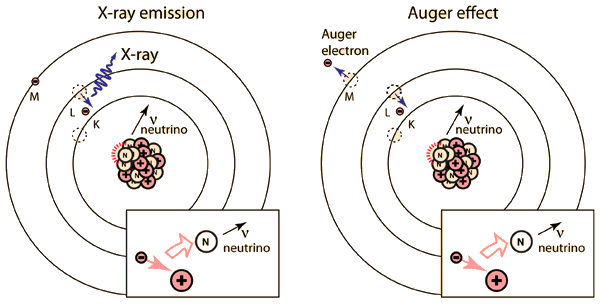
\includegraphics[scale=0.5]{img/ecrelax.png}
   \caption{oribital electon capture relaxation processes}
  \label{fig:ec1}
\end{figure}

Because electron capture occurs in (proton-rich) nuclei, and, subsequently, releases a X-Ray photon, the reaction is also sometimes written as

$$^{Z}X_{A}+\;e^{-}\rightarrow\;^{Z-1}X_{A}\;+\;h\nu_{X-ray}$$

(where Z is the total number of protons and neutrons, A the number protons, and $h\nu_{X-ray}$ is an X-ray photon)

Indeed, orbital electron capture is evidenced by high intensity x-rays and soft electrons.  In 1938, Luis W. Alvarez observed the x-ray signature of orbital electron capture in activated Titanium ($^{48}V$). Since then, electron capture has been observed in about 150 radioactive isotopes.


\subsubsection{Radiative Electron Capture}

In very rare cases, a gamma ray photon is emitted with the neutrino; this is called Radiative Electron Capture (REC) [10]. This can be thought of as a kind of Internal Bremsstrahlung radiation, caused by the electron accelerating toward the nucleus during capture. Recent, detailed rate calculations have elucidated the details [11].

\subsubsection{Effect of Chemical Environment of Electron Capture rate} 
The lightest element that electron capture has been observed in is $^{7}Be$ [3]. In fact, there is so little energy that the competing positron emission process (described below) is prohibited, and the half-life for electron capture is $\tau_{EC}\sim 50\;days$.

Being so light, and having such a large rate, electron capture in $^{7}Be$ can be slighlty modified by both changing the chemical environment and/or the external pressure [4-6]. In particular, in 2004, Ohtsuki et al demonstrated a change of 0.83%  by embedding Be in C-60 cages [6].

How could such changes occur ?

The rate of electron capture depends the electric density at the surface of the nucleus (the nuclear charge).   The electronic energy levels are in the eV range, so intense EM fields can alter the electronic structure and therefore slightly affect the rate. In contrast, the nuclear energy levels are in the keV to MeV region, and it is generally thought to be very difficult to impossible to effect. Of particular practical interest is using very large electric fields for accelerating Beta decay for disposing of nuclear waste [?].

\subsection{The Weak Interaction and V-A theory}

Orbital electron capture is mediated by the Weak interaction, described most concisely by the Fermi V-A (Vector Axial) theory [8].
The V-A theory is a simple phenomenological approach, readily amenable to numerical calculations.   Although it is now understood in terms of ElectroWeak Unification and can be derived from the Standard Model [9]. But we don't need all this machinery to do calculations.

V-A theory is used to compute cross sections for scattering experiments and decay rates for electron capture for various atoms and even in different environments, chemical and otherwise.  To properly describe any reaction, however, we need to understand what reactions we can apply the theory to, and the other competing reactions that might also occur.

\subsubsection{Electron Capture and other (weak) processes} 

The Weak interaction describes a variety of processes.  \emph{Neutron-rich} nuclei may become more stable as a result by undergoing one or more of the following:


\begin{itemize}
\item orbital electron capture $\;\;\;\;\;\;\;\;\;p^{+}+e^{-} \rightarrow n^{0}+\nu_{e}$

\item positon emission ($\beta^{+}$ decay) $\;p^{+}\rightarrow\;n^{0}+\;e^{+}\;+\;\nu_{e}$ 
\item or $\beta$ decay $\;\;\;\;\;\;\;\;\;\;\;\;\;\;\;\;\;\;\;\;\;\;\;\;\;\;\;\;\;n^{0}\rightarrow p^{+}+\;e^{-}\;+\;\bar{\nu_{e}}$
\end{itemize}

There are also several related reactions, including

\begin{itemize}
\item reverse electron capture  $\;\;\;\;\;\;\;n^{0}+\nu_{e}\rightarrow p^{+}+e^{-}$
\item free neutron decay  $\;\;\;\;\;\;\;\;\;\;\;\;\;\;\;n^{0}\rightarrow p^{+}+e^{-}+\bar{\nu_{e}}$ 
\item inverse beta decay  $\;\;\;\;\;\;\;\;\;\;\;\;\;\;\;p^{+}+\bar{\nu_{e}} \rightarrow n^{0}+e^{+}$
\end{itemize}



\subsubsection{Neutron decay}

By detailed balance,  reverse electron capture has the same rate as orbital electron capture,  but is more favorable energetically.  Indeed, inside the nucleus, the neutron is stable. Free neutron decay has mean lifetime of $\tau=881.5\pm1.5\;sec $, or about 15 minutes. 

In contrast, orbital electron capture by a free proton is unspokenof outside of a stellar environments. Even if the bare reaction could proceed, the reverse reaction would still dominate unless it is suppressed or is kinetically unfavorable. 

\subsubsection{Inverse Beta decay}

Electron capture is also sometimes called inverse $\beta$ decay, but, here, we mean this to be the scattering of a proton and an electron anti-neutrino.  It is characterized by emission of a positron. 

\subsubsection{Positron emission}

In particular, any high energy relativisitic process, we have to worry about positron creation.  We noted above, however, that in $^{7}Be$, the competing positron decay reaction can not occur because there is not enough energy.  Generally, this occurs at length scales below the Compton length of the electron, which, is smaller than we will need to consider.

\subsubsection{Internal Bremsstrahlung}

Electron capture and Beta decay events may also emit Bremsstrahlung (or so-called \emph{braking}) radiation, in the form of soft gamma rays[**]. this is 1000X less likely, but does occur.  In electron capture, the electron emits this as it \emph{accelerates} toward the nucleus, taking energy away from outbound neutrino.  The resulting gamma rays are called soft because they do not exhibit sharp spectral lines.  

\subsubsection{Rate calculations}

The electron capture rate can be computed using the Fermi VA-Theory [8,10].  The most basic calculations require a only specifying the electronic wavefunctions(s), averaging over the possible electron-proton momenta, and numerically integrating over the outbound neutrino momentum.  We describe this below.

The V-A theory is just second order perturbation theory.  It assumes an incoherent nuclear process, it is local, and that the interaction is phenomenological. It is treated as a simply a contact potential at the surface of the nucleus. Here, this means we only need to compute the nuclear charge--the electron density on the surface of the nucleus $\Vert\psi_{e}(R=0)\Vert$.  

More complicated calculations are used for larger nuclei, second order processes, etc. []  They only require modifications to treat either atomic electronic structure of reactant and product atoms, and/or specific considerations for nuclear internal conversion and other second order processes.

\subsection{Bare proton-electron capture}


We frequently write electron capture as if it were simply proton-electron capture

$$p^{+}+e^{-} \rightleftarrows n^{0}+\nu_{e}\;\;.$$

At zero energy, proton electron capture is not possible because it violates energy-momentum conservation. Theoretically, a free proton can could capture an electron from the continuum, but the interaction energy must be  above threshold for neutron production.  This is a huge amount of energy, although this happens regularly in accelerators.

Observing proton electron capture outside of an accelerator, \emph{on the desktop}, so to speak, would be an incredibly hard experiment because both final particles are neutral, and  the neutrino is extremely weakly interacting.

\subsubsection{Stellar Nucleosynthesis}

Bare proton-electron Capture is thought to occur in stars.  It is thought to drive the formation of primordial elements, and to occur in the forming of neutron stars [?].  For example, Bachall and coworkers have studied the electron capture rate in stellar media, and have computed the electron capture rate of $^{7}Be$ in the Sun [13].

 It is believed that ionized Hydrogen captures an electron during the core collapse supernovae and in neutron stars [14]; in fact, it is thought to create stellar instability.  At very high Temperatures, the proton electron collisions have sufficient energy to overcome the reaction barrier.  And while we usually characterize a star by it's temperature, these are also very dense systems, with $\rho\sim 10^6\;g\;cm^{-3}$.  In contrast, the smallest star has density $\rho\sim 10^{2}-10^{3}\;g\;cm^{-3}$ [?]  As important, the reverse reaction is prohibited because, inside the dense neutron star, it is impossible to create a new electron; the Fermi sea is 'full'.

So electron capture can occur by bare protons, but, presumably, only under extreme confinement (and with the reverse reaction is suppressed).

\section{Confinement Induced Electron Capture}

We pose the following Gedankenexperiment:  

Suppose we confine an electron and a bare proton as a particle-in-a-box of volume $L^3$.  What box size L will 'induce' electron confinement ?

We write this as

$$E_{box}+p^{+}+e^{-}\rightarrow n^{0}+\nu_{e}$$

where $E_{box}$ is the \emph{confinement energy}, which is induced by the box constraints. 

\subsubsection{Neutron post-reaction}

To prevent the reverse reaction, we assume that the free neutron subsequently combines with another proton, and gives us 2.2 GeV of energy in the process.  This post-process contributes to the power output, and prevents the reverse reaction.  Realistically, we expect this to happen at the maximum box size, at the energy threshold, where the outbound neutron has very low momentum and therefore a very small mean free path.  

\subsection{Compton length considerations}
The first obvious question is, should we use a classical or a relativisitic box?   

Most electron capture rate calculations use \emph{ab initio} classical wavefunctions [10, 12], perhaps with some relativisitic corrections to the electronic Hamiltonian [cite my book]

We can safely use a classical box as long as $L_{min} \ge \dfrac{1}{2\pi}\lambda_{e}$, where $\lambda_{e}$ is Compton wavelength of an electron [16-19].  The Compton wavelength sets the scale, accounting for both quantum mechanics and special relativity. [15]

$$\lambda_{e}=\dfrac{h}{m_{e}c}=\dfrac{e^{2}}{m_{e}c^{2}}$$

$$\lambda_{e}\approx2.426\times 10^{-12}\;m$$

For an electron, the minimum L is on the order of 0.004 Angstrom 
$$L_{min}\sim0.004\;\mathring{A}$$ 

In any high energy, relativisitic system, positrons can be produced; here it is through $\beta^{+}$-decay. This generally occurs at / below the Compton length. We are seeking the maximum box size which can induce electron capture, and we assume that, at the max, positron emission will be very rare.

We also assume that the electron wavefunction does not change appreciably during the interaction, so that we may use a very simplified form for the cross section ($\sigma$) and rate ($\Gamma$).  Again, this is reasonable for boxes $L\ge\lambda_{e}$.

So we use a classical box, with minimum size $L_{min}=0.004\;\mathring{A}$.  We compute the maximum size below.

\subsection{Theory}

\subsubsection{Particle production under the Weak interaction}

\begin{figure}
   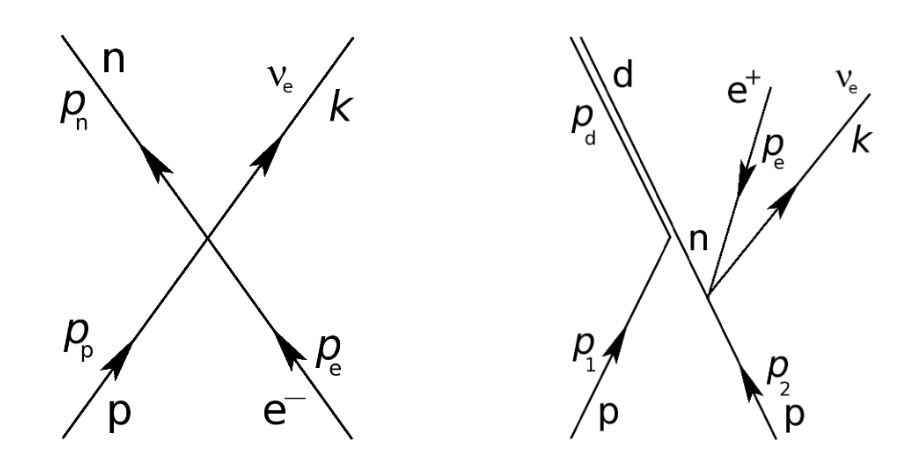
\includegraphics[scale=0.25]{img/feynman.png}
   \caption{Particle production process}
  \label{fig:ppp}
\end{figure}

Electron capture is mediated by the Weak Interaction, through the particle production process, given by the 4-point Interaction (see Figure \ref{fig:ppp}).   It requires 0.511 MeV energy to overcome the reaction barrier, which, here, is \emph{provided} by the box. 

\subsubsection{Hamiltonian}

The Hamiltonian for the V-A theory is [?]

$$\mathcal{H}(x)=-\dfrac{G_{F}}{\sqrt{2}}\left[J^{\mu}(x)L^{+}_{\mu}(x)+h.c.\right]$$

where $J_{\mu}$ and $L_{\mu}$ are the Hadron and Lepton currents, resp, and are given by

$$J_{\mu}=\bar{u}_{n}\gamma_{\mu}(1+\lambda\gamma_{5})u_{p}$$

$$L_{\mu}=\bar{u}_{\mu}(1+\gamma_{5})u_{e}$$

where $u_{n},u_{p},u_{e},u_{\nu}$ are Dirac Spinors.

$G_{F}$ is the Universal Fermi Weak Coupling Constant, and $\lambda=-\dfrac{G_{A}}{G_{V}}$, which is determined by experiment (and subject to minor changes).  $G_{V}$ is the Axial-Vector Weak Coupling Constant, and $G_{A}$ is the vector weak coupling
constant.  The most recent value is $G_{V}=?1.27590^{+0.00409}_{?0.00445}$, and $G_{A}=1$ "under the conserved vector current (CVC) hypothesis of the Standard Model" [22].
 
\subsubsection{Transition Rates and Power Calculations}

We want to compute the power generated by confined electron capture, as a funciton of the box size (L)
We need the  rate of electron capture, $\Gamma_{EC}$, which is given by Fermi's Golden Rule 

$$\Gamma_{EC}=\Gamma_{fi}=2\pi|\mathcal{M}_{fi}|^{2}\rho(E_{f})$$

where the matrix element $\mathcal{M}_{fi}$and the density of states $\rho(E_{f})$ must be Lorentz Invariant (L.I.)

The matrix elements are 
$$\mathcal{M}_{fi}=\left<\Psi_{final}\big\vert\mathcal{H}\big\vert\Psi_{final}\right>$$


\subsubsection{VA Matrix Elements}

We use a slghtly different convention for the matrix elements, multiplying by $G_{V}$, giving

The matrix elements $\mathcal{M}_{fi}$ are

$$\mathcal{M}_{fi}=\dfrac{G_{F}}{\sqrt{2}}\bar{u}(p_{n},s_{n})(G_{V}-G_{A}\gamma^{5})\gamma^{\mu}u(p_{p},s_{p})\times\bar{u}(k,s_{k})\gamma_{u}(1-\gamma^{5})u(s_{e},p_{e})$$


We use Dirac 4-Spinors

$$\bar{u}(p_{n},s_{n}),u(p_{p},s_{p}),\bar{u}(k,s_{k}),u(s_{e},p_{e})$$
where

$$s_{n}, s_{p},s_{e},s_{k}$$ 

are 2-component spin vectors for the neutron, proton, electron, and electron neutrino, resp. 

The Dirac spinors assume the standard energy normalization $\dfrac{1}{\sqrt{2E}}$.

The $\gamma$ are 4-component Gamma matrices, and  $(\cdots\gamma^{\mu}\cdots\gamma_{u}\cdots)$ is the Einstein summation convention.


\subsubsection{Cross Section}

The cross section for the process is given by 

$$d\sigma_{ep}=\left(\dfrac{1}{2\pi}\right)^{2}\dfrac{\sum_{fi}\big\vert\mathcal{M}_{fi}\big\vert^{2}}{16\;\big\vert\mathbf{k}\cdot(E{_n}\mathbf{k}-k^{0}\mathbf{p}_{n})\big\vert}\dfrac{k^{3}p_{e}d\Omega_{k}}{\big\vert\mathbf{p}_{e}\cdot(E_{p}\mathbf{p}_{e}-E_{e}\mathbf{p}_{e})\big\vert}$$

Notice that when applying the VA theory this way, we assume that the electron-proton interaction is a contact potential, operating at the surface of the nucleus, and that the underlying quantum process is incoherent.  

\subsubsection{Particle-in-the-box Wavefunctions}


We treat the electron, proton pair as classical particle-in-a-box.

$$\psi_{ep}(\mathbf{x})=\left(\dfrac{2}{L}\right)^{\frac{3}{2}}cos\left(\dfrac{\pi x}{L}\right)cos\left(\dfrac{\pi y}{L}\right)cos\left(\dfrac{\pi z}{L}\right)$$

expressions for momentum

Because the VA theory assumes an incoherent process, the electron, proton wavefunction is usually factored as an electron wavefunction, with a point-particle in the center

$$\psi_{ep}(\mathbf{x})=\psi_{p}(0)\psi_{e}(\mathbf{x})$$

We only consider the  ground state $\psi_{ep}^{0}$ wavefunction.


We note, in \emph{ab initio} electronic structure calculations, it is now generally possible to treat the Hydrogen proton wavefunction explicitly, and to treat the electron-proton coupling at the level of Hartree Fock [my book, 12].  This has proved useful for describing isotope effects on electronic structure [?]

Here, we treat the confined electron, proton pair in the c.m. frame so that the 3-momentum of the electron and proton related
$$\mathbf{p}_{e}=\mathbf{p}_{pe}$$
$$\mathbf{p}_{p}=-\mathbf{p}_{pe}$$

\subsubsection{comment on our approach}

We note that Blatt and Weisskopf [20] describe the fermi VA theory in the non-relativisitic limit.  Here, they use classical plane wave solutions $(e^{i\mathbf{p}\mathbf{x}})$, with just box normalization $(\frac{1}{L^{3}})$.  In contrast, we use the full classical particle-in-the-box wavefunctions, and analyze the problem just above the Compton scale using the low order VA theory.

\subsubsection{Rate of Confined Electron Capture}

Given the computed Dirac 4-vectors, we can compute the rate of electron capture using the VA-theory, for a given set of vectors

For the process

$$E_{box}+p^{+}+e^{-}\rightarrow n^{0}+\nu_{e}$$

The rate $\Gamma_{EC}$ of electron capture is determined by multiplying the cross section by the incident velocity $\mathbf{v}_{in}$ and the the electronic wavefunction at the origin 

$$\Gamma_{EC}=\big\vert\Psi(0)\big\vert^{2}\mathbf{v}_{in}\sigma_{EC}$$

This gives :

$$d\lambda_{ep}=\left(\dfrac{1}{2\pi}\right)^{2}\dfrac{\sum_{fi}\big\vert\mathcal{M}_{fi}\left[p_{ep}\rightarrow i\nabla)\right]\psi_{ep}(\mathbf{x})\big\vert_{\mathbf{x}=0}\big\vert^{2}}{16E_{p}E_{e}\;\big\vert\mathbf{k}\cdot(E{_n}\mathbf{k}-k^{0}\mathbf{p}_{n})\big\vert}k^{3}d\Omega_{k}$$


\subsubsection{Relativistic Kinematics and Energetics}
For consistency with the particle production process, we treat all kinematics and energetics relativistically.  

[ explain how we got here]

We have

$$E^{2}_{e}=m^{2}_{e}+3\left(\dfrac{\pi}{L}\right)^{2}$$ 

$$E^{2}_{p}=M^{2}_{p}+3\left(\dfrac{\pi}{L}\right)^{2}$$

The threshold Kinetic energy in the center of momentum (c.m.) frame is given as

$$EKe_{min}:\;\;K_{e}=E_{e}-m_{e}=\dfrac{(M_{n}-m_{e}+m_{\nu})^{2}-M^{2}_{p}}{2(M_{n}+m_{\nu})}$$
 
Giving the minimum momentum as

$$pmin:\;\;\mathbf{p}_{min}=\sqrt{(K_{e}+m_{e})^{2}-m_{e}^{2}} $$

Of course, the proton rest frame is approximately the electron rest frame, but it should be mentioned that the in the electron rest frame, the threshold kinetic energy is 2000X greater.  Therefore, it is assumed that the energy transfer to induce electron capture is in the c.m. frame of the (e,p) pair.

The total energy in the c.m. frame is

$$E_{tot}=E_{n}-E_{e}$$

For the final state, the neutrino kinetic energy is

$$K_{\nu}=k^{0}-m_{\nu}=\dfrac{(E_{p}+E_{e}-m_{\nu})^{2}-M^{2}_{n}}{2(E_{p}+E_{e})}$$

and the neutron kinetic energy is

$$K_{n}=E_{n}-M_{n}=\dfrac{(E_{p}+E_{e}-M_{n})^{2}-m^{2}_{\nu}}{2(E_{p}+E_{e})}$$

\end{document}  




[**] We refer to photons emitted directly from the nucleus as gamma rays, whereas those emitted from atomic electrons are called x-rays.    The naming convention reflects the different origins.







